\documentclass[runningheads]{llncs}

% ---------------------------------------------------------------
% Include basic ECCV package
 
% TODO REVIEW: Insert your submission number below by replacing '*****'
% TODO FINAL: Comment out the following line for the camera-ready version
\usepackage[review,year=2024,ID= 12215]{eccv}
% TODO FINAL: Un-comment the following line for the camera-ready version
%\usepackage{eccv}

% OPTIONAL: Un-comment the following line for a version which is easier to read
% on small portrait-orientation screens (e.g., mobile phones, or beside other windows)
%\usepackage[mobile]{eccv}


% ---------------------------------------------------------------
% Other packages

% Commonly used abbreviations (\eg, \ie, \etc, \cf, \etal, etc.)
\usepackage{eccvabbrv}

% Include other packages here, before hyperref.
\usepackage{graphicx}
\usepackage{booktabs}

% The "axessiblity" package can be found at: https://ctan.org/pkg/axessibility?lang=en
% Will be Un-Commented at later releases
%\usepackage[accsupp]{axessibility}  % Improves PDF readability for those with disabilities.



% ---------------------------------------------------------------
% Hyperref package

% It is strongly recommended to use hyperref, especially for the review version.
% Please disable hyperref *only* if you encounter grave issues.
% hyperref with option pagebackref eases the reviewers' job, but should be disabled for the final version.
%
% If you comment hyperref and then uncomment it, you should delete
% main.aux before re-running LaTeX.
% (Or just hit 'q' on the first LaTeX run, let it finish, and you
%  should be clear).

% TODO FINAL: Comment out the following line for the camera-ready version
\usepackage[pagebackref,breaklinks,colorlinks,citecolor=eccvblue]{hyperref}
% TODO FINAL: Un-comment the following line for the camera-ready version
%\usepackage{hyperref}

% Support for ORCID icon
\usepackage{orcidlink}


% Support nth ordering
% Can be Commented if needed
\usepackage[super]{nth}

\begin{document}

% ---------------------------------------------------------------
% TODO REVIEW: Replace with your title
\title{SATURN: Splitting Approach on Tensorized Ubiquitous Regression Networks} 

% TODO REVIEW: If the paper title is too long for the running head, you can set
% an abbreviated paper title here. If not, comment out.
\titlerunning{SATURN}

% TODO FINAL: Replace with your author list. 
% Include the authors' OCRID for the camera-ready version, if at all possible.
\author{
Amir Mohammad Kharazi\inst{1}
%\orcidlink{0000-1111-2222-3333}
\and
Mohammad Badzohreh\inst{2,3}
%\orcidlink{1111-2222-3333-4444} 
\and
Mansoor Rezghi\inst{3}
%\orcidlink{2222--3333-4444-5555}
}

% TODO FINAL: Replace with an abbreviated list of authors.
%\authorrunning{F.~Author et al.}
\authorrunning{
	A.~M.~Kharazi et al. 
	M.~Badzohreh et al.
	M.~Rezghi}
% First names are abbreviated in the running head.
% If there are more than two authors, 'et al.' is used.

% TODO FINAL: Replace with your institution list.
\institute{Tarbiat Modares University, Iran\\ \url{https://en.modares.ac.ir/} 
%\and
%Springer Heidelberg, Tiergartenstr.~17, 69121 Heidelberg, Germany
%\email{lncs@springer.com}\\
%\url{http://www.springer.com/gp/computer-science/lncs} \and
%ABC Institute, Rupert-Karls-University Heidelberg, Heidelberg, Germany\\
%\email{\{abc,lncs\}@uni-heidelberg.de}
}

\maketitle


\begin{abstract}
  \textit{Fully Connected} (FC) layers are often used in many neural network architectures, such as \textit{Convolutional Neural Networks} (CNNs), which usually flatten the data before feeding it to the FC layers. Despite empirical success, some drawbacks include the changing of topological structure and the number of required parameters. Methods like the \textit{Tensor Contraction Layer} (TCL) and \textit{Tensor Regression Layer} (TRL) are capable candidates to use instead of FC layers, which preserve the multilinear structure of data as well as reduce the cost of execution. To exploit their capability even further, our method uses specific splitting approaches to generate thinner, higher dimensional tensors from the original data to reduce the cost by a greater factor while also maintaining accuracy. Our experiments on CIFAR10 and MNIST, applied to known models such as ResNet, VGG, and other typical CNNs, demonstrate our method's ability to reduce the cost compared to previous models and their TCL-TRL adaptation while also maintaining accuracy.
  %\keywords{We would like to encourage you to list your keywords within
  %the abstract section}
  \keywords{
  	Machine Learning, Tensorized Regression Layer, Tensorized Contraction Layer, Patching and Splitting, Tensor Methods, Low-Rank Approximation
  }
\end{abstract}


\section{Introduction}
\label{sec:intro}

Conventional Neural Networks, especially those that are applied to images such as \textit{Convolutional Neural Network} (CNNs), often consist of two main parts: One that is responsible to extract features from the input data, and the other part is a \textit{MultiLayer Perceptron} (MLP) which Maps the extracted features to the desired space. Despite the importance of data and their spatial relationship, maintaining their topological structure is often discarded since many known CNNs like ResNet or VGG, seem to work fine as they are; However in cases where these structures are more important than the others such as MRI, It is crucial to adapt the known networks to work without destroying the multi-linear structure of the data.

Multi-linear or Multi-modal structures have always existed in many natural datasets and we can represent these using Tensors; Images could be considered as a \nth{3} orders tensors with width, height and the color channels as the corresponding 3 modes, the same could be considered for videos as \nth{4} order tensor with an extra time mode. In practice, many of the natural datasets can be considered as tensors which then requires the tensor expansion to the linear algebra. 

Considering the new advances in \textit{Deep Neural Networks} (DNNs) and their applications to computer vision such as image recognition, image segmentation, image generation, video generation, vision transformers, etc $\dots$; most architectures still flatten the data before using them on MLPs which not only destroys the natural structure of the data but also increase the number of parameters needed for the model. 

Images as the prime example of data used in vision machine learning tasks are considered \nth{3} order tensors which require their own algebra to be applied when fed to the MLPs (convolution layers are already designed to work on tensors). \textit{Fully Connected} (FC) layers used in many architectures are the main culprit behind vectorizing the data and the number of parameters. To alleviate the situation, a better replacement for FC layers is needed which not only preserves the current model's accuracy but also reduces the number of required parameters and does not destroy the structure of data. 

Some works have been done to address these issues which will be discussed in Section 2. Our method provides a better solution based on one of the previous works and the experiments on CIFAR10 and MNIST applied to known architectures, ResNet and VGG, and typical CNNs proves our superiority. Using a splitting method, to split the original tensor along its modes into smaller tensors and stacking them into a newer, thinner and higher dimensional tensor we reduced the number of parameters while also maintaining the accuracy.

\section{Related Works}
\label{sec:related-work}

Several prior papers address the importance of using tensors and preserving the natural structure, one notable recent work is Tensor Regression Networks \cite{kossaifi2020tensor} by Kossaifi. They used a \textit{Tensor Regression Layer} (TRL) and \textit{Tensor Contraction Layer} (TCL) to preserve the structure of data as they are moving across the network while also reduce the number of parameters. Their method surprisingly achieved the near similar accuracy as its FC network with more than \%65 space saving. TRL and TCL will be discussed in section 3, and they are used as the base of our method. Unfortunately, one of the biggest issues with TCL and TRL is their inadequate implementations. They are theoretically required less parameters than their FC versions; However they often perform poorly in terms of the actual execution time as their implementations are based on folding and unfolding tensors which is not very well understood in the famous python libraries like PyTorch and is hard to calculate their backpropagation.

\section{Mathematical Prequisions}
\label{sec:mathematical-prequisions}
Given the tensorized nature of our methods, it is required to be familiar with basic tensor methods. In this section, we introduce some of the tensor notation and methods used in our model.

\subsection{Notation}
\label{subsec:notation}
For a 3-order tensor $T\in \mathbb{R}^{I_0\times I_1\times I_2}$, there are 3 modes with respected sizes $I_0$, $I_1$, and $I_2$. 
Its $T_{i_0, i_1, i_2}$ 
\textbf{element}
is 0-order tensor (scalar), $(i_0, i_1, i_2)$. 
\textbf{Slices} of its first and second modes are 2-order tensors (matrices) $M$ and are denoted by two colons, $T_{:,:,i_2}$. 
\textbf{Fibers} of its first mode are 1-order tensors (vectors) $V$ and are denoted by a colon, $T_{:, i_1, i_2}$.

\subsection{Tensor n-mode unfolding}
\label{subsec:tensor-unfolding}
Given a tensor 
$T\in \mathbb{R}^{I_0\times I_1\times \dots \times I_N}$,
its n-mode unfolding is a matrix defined
\linebreak 
as $T_{\left[n\right]} \in \mathbb{R}^{I_n \times \left(I_0\times \dots I_{n-1}\times I_{n+1}\times \dots \times I_N\right)}$. Mapping of elements are done via :

\begin{align}
	\label{eq:unfolding}
	&(i_0, \dots, i_n,\dots,i_N) \longrightarrow (i_n,j)\\
	&\text{where } j = \sum_{\substack{p=0 \\ p\neq n}}^{N} I_p \prod_{\substack{l=p+1 \\ l\neq n}}^{N} I_l
\end{align}

\subsection{Tensor Vectorization}
\label{subsec:tensor-vectorization}
Given a tensor 
$T\in \mathbb{R}^{I_0\times I_1\times \dots \times I_N}$, its vectorization is defined as $Vec(T) \in \mathbb{R}^{(I_0\times \dots \times I_N)}$. Mapping of elements are done via :

\begin{align}
	\label{eq:vectorization}
	&(i_1,\dots,i_N) \longrightarrow j\\
	&\text{where } j = \sum_{\substack{p=0}}^{N} I_p \prod_{\substack{l=p+1}}^{N} I_l
\end{align}

\subsection{Tensor $n$-mode product}
\label{subsec:tensor-nmode-product}
Given a tensor 
$T\in \mathbb{R}^{I_0\times \dots\times I_n \times \dots \times I_N}$, its $n$-mode product with matrix
\linebreak
 $M \in \mathbb{R}^{J_n \times I_n}$ is defined as $ (T \times_n M) \in \mathbb{R}^{I_0\times \dots\times J_n \times \dots \times I_N}$. Tensor $n$-mode product is a very useful method used in many tensor related operations as the foundation and many tensor decomposition and contractions are done via multiple $n$-mode products. Mapping of elements are done via : 
 % change mapping of elements to something else 
 
 \begin{align}
 	\label{eq:nmode-product}
 	&i_0,i_1,\dots,i_{n-1},j_n,i_{n+1},\dots,i_N \longrightarrow j\\
 	&\text{where } j = \sum_{i_n = 0}^{I_n} T_{i_0,\dots,i_N} M_{j_n,i_n}
 \end{align}
 
 
 
 Tensor $n$-mode product can be expressed as the dot product of two matrices, $M \in \mathbb{R}^{J_n \times I_n}$ and $T_{\left[n\right]}$ from \ref{subsec:tensor-unfolding}. 
 
 \begin{align}
 	\label{eq:nmode-product-matrix}
 	(T \times_n M ) = MT_{\left[n\right]} \in \mathbb{R}^{I_0\times \dots\times J_n \times \dots \times I_N}
 \end{align} 


\subsection{Tensor Contraction}
\label{subsec:tensor-contraction}
%Or Known as "Generalized Inner Product" 


\section{Tensor Regression Network}
\label{sec:tensor-regression-network}
Tensor Regression Networks are introduced by Kossaifi as mentioned in Section 2. Given a MLP, there are two ways interpret FC layers: One is to consider them as a feature extraction layer which is usually all of the non classifier layers, And another way is consider them as regression layers which are basically the classifier layers. Given the purpose of the network and its author, they can be used differently. Figure 1 presents a very simple MLP that is being used after some convolution layers.


\begin{figure}
	\centering
	
\includegraphics[scale=0.4]{pictures/fig1.jpg}
	\caption{will be filled later}
\end{figure}


\subsection{TCL}
\label{subsec:tcl}
Tensor Contraction Layer is a form of feature extraction and could also be used for embedding. The prime idea behind TCL is Tucker decomposition. Via multiplying matrices to each mode of the input tensor, we can obtain a denser (dependent of the shape of the matrices) tensor. Figure 2 demonstrate the TCL process on a \nth{3} order tensor. 

Considering an input tensor $X$ of size 
$(S_0,I_0,I_1,\dots,I_N)$ and a size 
\linebreak 
$(R_0,R_1,\dots,R_N)$ TCL, where $S_0$ is the size of the batch and $(I_i,R_i)$ is the shape of the matrix applied to mode $i$ of the tensor; The number of parameter is 
$\sum_{i=0}^{N}I_i\times R_i$ and the output tensor size would be 
$(S_0, R_0,R_1,\dots,R_N)$. Compared to the FC version where the simple regression between these two tensors would require $\prod_{i=0}^{N}I_i\times R_i$ parameters.


\begin{figure}
	\centering
	
\includegraphics[scale=0.4]{pictures/fig2.jpg}
	\caption{will be filled later}
\end{figure}

\subsection{TRL}
\label{subsec:trl}
Tensor Regression Layers is a form of replacement for the original FC layers and regression layers. The simple regression that is the foundation of MLP is a trivial generalized inner product of $W$ (Weight Tensor) with the $X$ (Input tensor). The idea behind TRL is to reconstruct $W$ from a low rank approximation of its via tucker decomposition. Figure 3 presents the TRL application in MLP. For the sake of simplicity, we considered a binary classification problem where the output of the inner product is a scaler. Similarly, if the desired output is a vector or even a tensor, $W$ will be a higher dimensional tensor itself to generate each mode of the output. 

Considering an input tensor $X$ of size 
$(S_0,I_0,I_1,\dots,I_N)$, a size 
\linebreak 
$S_0 \times O$ output $Y$, and a size 
$(R_0,R_1,\dots,R_N, R_{N+1})$ TRL with bias $b$ of size $O$  such that 
$Y = <X,W>_N + b$; The number of required parameters would be 
$\prod_{i=0}^{N}R_i + R_{N+1}\times O + \sum_{i=0}^{N} R_i\times I_i$. Compared to the FC version where the number of parameters is $O\times\prod_{i=0}^{N}I_i$.


\begin{figure}
	\centering
	
\includegraphics[scale=0.4]{pictures/fig3.jpg}
	\caption{will be filled later}
\end{figure}


\section{Splitting Approach}
\label{sec:splitting-approach}

Impressed by the vision transformers patching and down sampling methods, we can transform out input tensor into a thinner higher dimensional tensor that not only reduces the number of parameters but also maintain the accuracy. Given the splitting scheme, the newly made tenser has better physical interpretation than the flattened data. We introduced two splitting scheme, both of them are useful and could be used differently according to the designer of the network. Figure 4 demonstrate the general splitting outline. Given a \nth{3} order tensor, if we split across each mode, the output is a \nth{6} order tensor where the first 3 modes correspond the split index, and the next 3 modes are the data.

\begin{figure}
	\centering
	
\includegraphics[scale=0.1]{pictures/fig4.jpg}
	\caption{will be filled later}
\end{figure}

\subsection{Attached Splitting}
\label{subsec:attached-approach}

In attached splitting, every split is continues, that is if mode  $I_i$ of the input tensor $X$ with length $n$ is to be split into 2 parts, then the split indices are $(0,\frac{n}{2})$ and $(\frac{n}{2}, n)$. Figure 5 demonstrate the splitting process on a matrix. This is the simple splitting method seen on many vision machine learning models via different names. 

\begin{figure}
	\centering
	\includegraphics[scale=0.4]{pictures/fig5.jpg}
	\caption{will be filled later}
\end{figure}

\subsection{Compressed Splitting}
\label{subsec:copressed-splitting}

In compressed splitting, we incorporate the idea behind down sampling, that is if mode $I_i$ of input tensor $X$ with length $n$ were to be split into 2 part , different to the attached splitting, the indices are even-odd combinations; That is $\left\{
t | t \in (0,n) \land \frac{t}{2}=0
\right\}$
and 
$\left\{
t | t \in (0,n) \land \frac{t}{2}=1
\right\}$
splits.

\begin{figure}
	\centering
	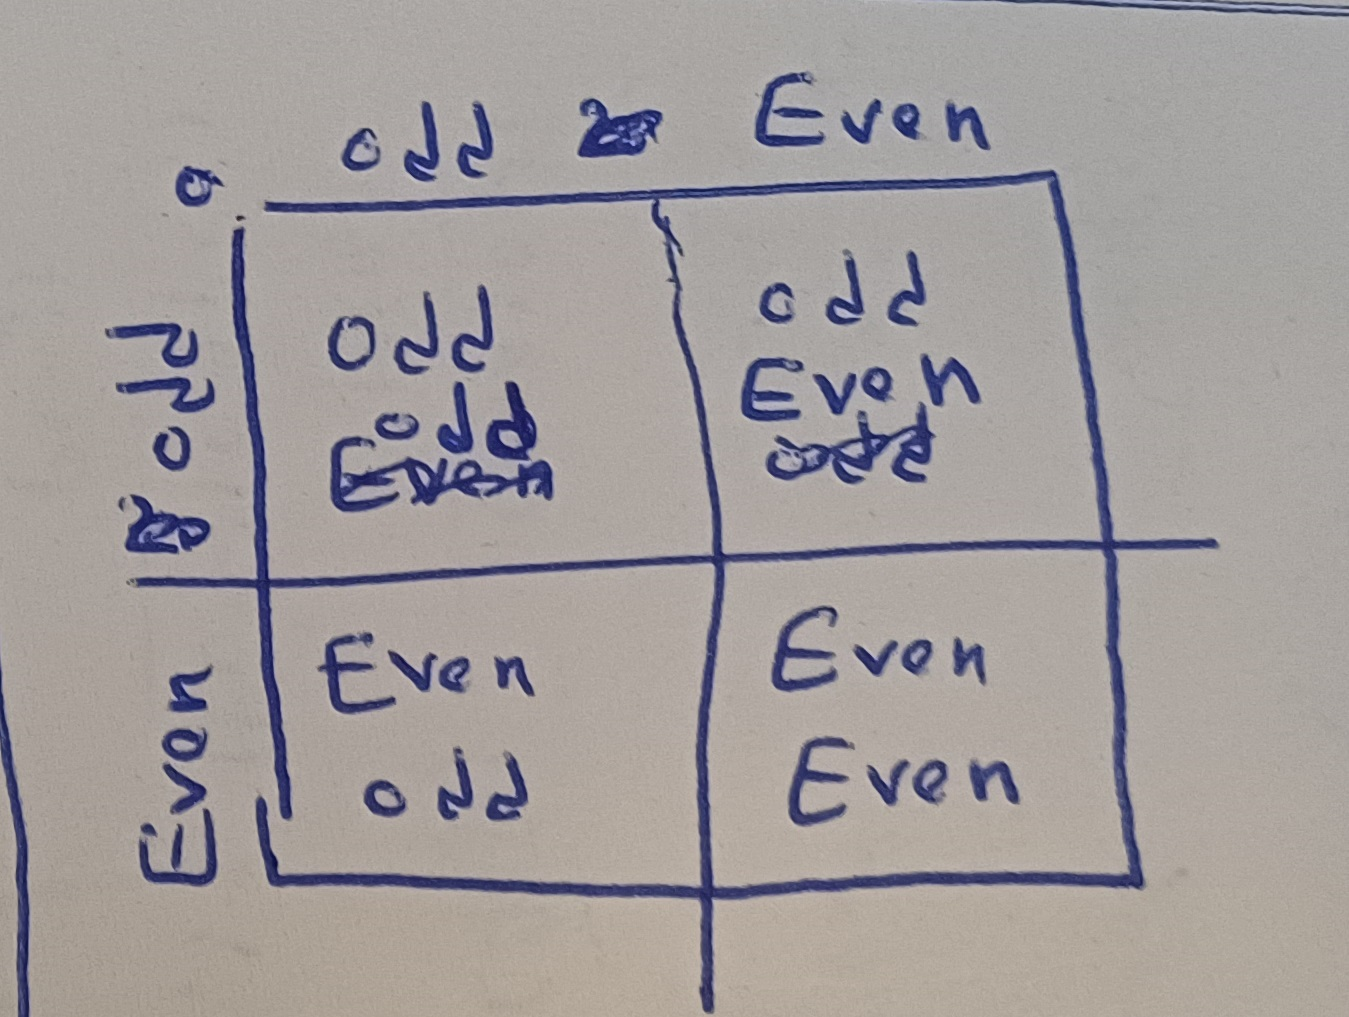
\includegraphics[scale=0.4]{pictures/fig6.jpg}
	\caption{will be filled later}
\end{figure}


\subsection{Method Analysis}
\label{subsec:method-analysis}
Considering a input tensor $X$ of size
$(S_0,I_0,I_1,\dots,I_N)$
, The splits on each mode except the batch mode would result in the tensor $\hat{X}$ of size
\linebreak
$(S_0, L_0,L_1,\dots,L_N, \frac{I_0}{L_0}, \frac{I_1}{L_1}, \dots, \frac{I_N}{L_N})$.

In case of TCL, Since $L_i$s are usually small, the number of parameters required for them are also small and is $\sum_{i=0}^{N}L_i\times r_i$ where $r_i$ is also small; Similarly, $\frac{I_i}{L_i}$ is smaller than $I_i$ so the desired $\hat{R}_i$ is smaller than the original $R_i$ and the total number of parameters is 
$\sum_{i=0}^{N}L_i\times r_i + \sum_{i=0}^{N}\frac{I_i}{L_i} \times \hat{R}_i$.

In case of TRL, the same logic as TCL could also be applied. The total number of parameters in a new TRL is 
$\prod_{i=0}^{N}r_i + \prod_{i=0}^{N}\hat{R}_i + \sum_{i=0}^{N}L_i\times r_i + \sum_{i=0}^{N}\frac{I_i}{L_i}\times \hat{R}_i + \hat{R}_{N+1}\times O$. 


\section{Experiment}
\label{sec:experiment}


\section{Conclusion}
The paper ends with a conclusion. 

%\clearpage\mbox{}Page \thepage\ of the manuscript.
%\clearpage\mbox{}Page \thepage\ of the manuscript.
%\clearpage\mbox{}Page \thepage\ of the manuscript.
%\clearpage\mbox{}Page \thepage\ of the manuscript.
%\clearpage\mbox{}Page \thepage\ of the manuscript. This is the last page.
%\par\vfill\par
%Now we have reached the maximum length of an ECCV \ECCVyear{} submission (excluding references).
%References should start immediately after the main text, but can continue past p.\ 14 if needed.
%\clearpage  % TODO REVIEW/FINAL: This \clearpage needs to be removed from both review and camera-ready versions.


% ---- Bibliography ----
%
% BibTeX users should specify bibliography style 'splncs04'.
% References will then be sorted and formatted in the correct style.
%
\bibliographystyle{splncs04}
\bibliography{main}
\end{document}
